Veamos finalmente, algunas t\'ecnicas de posprocesamiento para im\'agenes satelitales que nos ayudaran a mejorar los valores extraidos y conocer la incerteza en su estimaci\'on. Son nuestros objetivos:

\begin{itemize}
  \item Aplicar filtros modales a las clasificaciones para eliminar p\'ixeles aislados.
  \item Calcular la presici\'on total para la clasificaci\'on y las precisiones del usuario y productor.
  \item Estimar el error de las superficies calculadas a partir de la imagen clasificada.
\end{itemize}

Vamos a usar los paquetes \texttt{raster}, \texttt{rgdal}, \texttt{RStoolbox} y \texttt{rasterVis}.

\section{Filtrado de clasificaciones}

Luego de clasificar una imagen es necesario aplicar un filtro que permita eliminar p\'ixeles aislados. Al hacerlo, podremos descartar, p\'ixeles de ciudad en el medio de la selva o de selva en medio de la ciudad. \'Esta es otra forma de incorporar el contexto espacial a nuestras clasificaciones
\begin{exa}
  Veamos como aplicar un filtro por moda a una imagen clasificada. Comencemos cargando una imagen clasificada en R

  \begin{lstlisting}
      mlc.2016 = raster("raster_data/processed/mlc2016")
  \end{lstlisting}

  Para aplicar el filtro de 3x3 creamos una matriz de dicha dimensi\'on y usamos el comando \texttt{focal} con la funcion \texttt{modal}

  \begin{lstlisting}
    colores = c('#b2df8a','#33a02c',
                '#fdbf6f','#ff7f00',
                '#fb9a99','#e31a1c',
                '#a6cee3','#1f78b4')
    window <- matrix(1,nrow=3, ncol=3)
    mlc.3x3.2016 <-focal(mlc.2016,w=window,fun=modal)
    writeRaster(mlc.3x3.2016,"raster_data/processed/mlc3x3-2016", datatype = "INT1U", overwrite=TRUE)
    plot(mlc.3x3.2016,col=colores)
  \end{lstlisting}

  En el caso de un filtro por moda, estamos cambiando el valor del p\'ixel por la moda entre los que lo rodean. Podemos en este caso mostrar las im\'agenes con y sin el filtro juntas (figura \ref{fig:3x3}).

  \begin{lstlisting}
    plot(stack(mlc.2016, mlc.3x3.2016),col=colores)
  \end{lstlisting}

  \begin{figure}[h!]
    \centering
    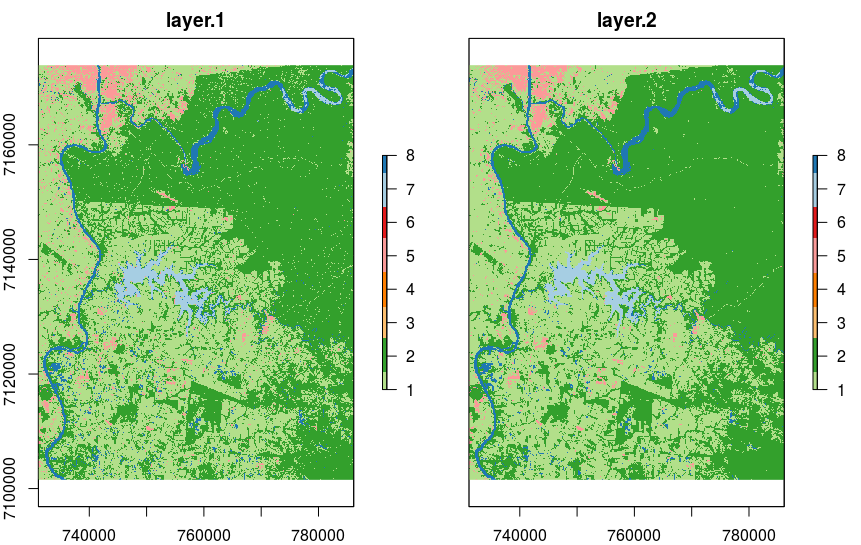
\includegraphics[scale=0.4]{filtro3x3.png}
    \caption{Imagen de la clasificaci\'on con y sin filtro con una ventana de 3x3.}
    \label{fig:3x3}
  \end{figure}
\end{exa}

\begin{act}
    Aplique filtros de 5x5 y 7x7 a la imagen. ¿Qu\'e problemas desaparecen? ¿Qu\'e dificultad introducen?
\end{act}

\begin{act}
    Aplique el filtro de 3x3 a la imagen correspondiente al año 2000.
\end{act}

\section{Validaci\'on de la clasificaci\'on}

El segundo procesamiento pos-clasificaci\'on, y tal vez el mas importante, es el c\'alculo de la matriz de confusi\'on para nuestra clasificaci\'on. Lo haremos en dos partes: crearemos primero el set de datos para la validaci\'on y luego lo usaremos para calcular la matriz de confusi\'on.

\begin{exa}
  Veamos como crear un set de puntos aleatorios de muestreo con QGIS. En \'este caso, utilizaremos como unidad de muestreo al p\'ixel, pero de forma similar pueden usarse pol\'igonos o grupos de pol\'igonos.

  Comenzamos abriendo la imagen \file{mlc3x3-2016} en QGIS. Luego vamos a vectorizar la clasificaci\'on utilizando la herramienta \menu{Raster, Conversi\'on, Poligonizar}. Guardamos el archivo como \file{2016-3x3.shp} en la carpeta de \file{vector\_data} poniendo en nombre del campo \menu{MC\_ID} (figura \ref{fig:poligon}).

  \begin{figure}[h!]
    \centering
    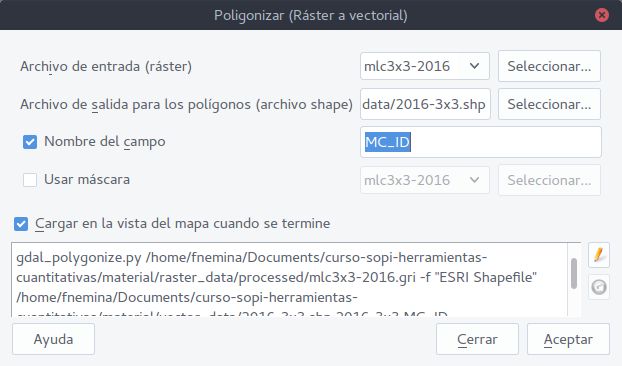
\includegraphics[scale=0.4]{poligon.png}
    \caption{Herramienta de poligonizaci\'on}
    \label{fig:poligon}
  \end{figure}

  Vamos luego a \menu{Herramientas de gesti\'on de datos, Dividir capa vectoria} y guardamos los vectores en la carpeta \file{vector\_data,split} (figura \ref{fig:split}).

  \begin{figure}[h!]
    \centering
    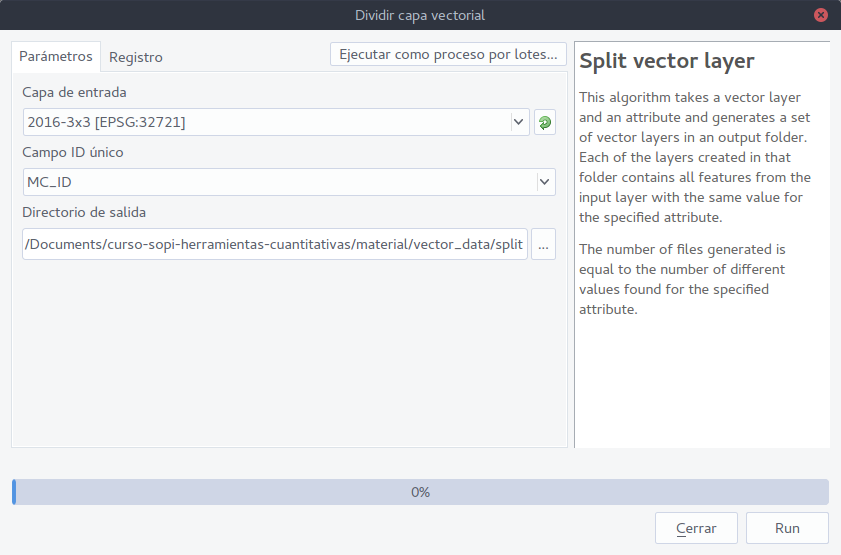
\includegraphics[scale=0.4]{split.png}
    \caption{Herramienta de divisi\'on de capa vectorial.}
    \label{fig:split}
  \end{figure}

  Cargamos las capas en QGIS. En \menu{Herramientas de investigacion, Puntos aleatorios en los limites de la capa} hacemos click en el bot\'on \menu{Ejecutar proceso por lotes}. Luego hacemos click en el bot\'on con los tres puntos y elegimos \menu{Seleccionar del sistema de archivos}.  Seleccionamos cada capa. En n\'umero de puntos ponemos la cantidad correspondiente a cada categor\'ia.

  Para calcular dicha cantidad usamos el comando \texttt{freq.2016 <- freq(mlc.3x3.2016)}  para conocer las frecuencias de aparici\'on de cada categor\'ia y luego con el comando  \texttt{freq.2016[,2] <- round(freq.2016[,2]/sum(freq.2016[,2])*250+50)} distribuimos  los p\'ixeles en cada categoria con 50 fijos y 250 seg\'un la frecuencia de aparici\'on.
  Los repartimos en la imagen con una distancia de separaci\'on m\'inima de 100m (figura \ref{fig:dots}).

  \begin{figure}[h!]
    \centering
    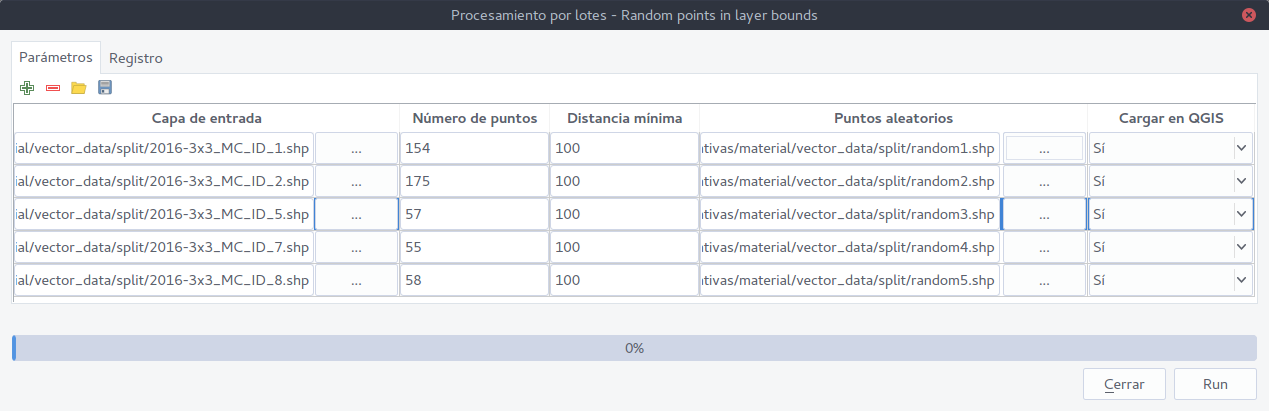
\includegraphics[scale=0.3]{random-dots.png}
    \caption{Herramienta de creaci\'on de puntos aleatorios.}
    \label{fig:dots}
  \end{figure}

  Elegimos luego en que carpeta guardar los puntos aleatorios y hacemos click en aceptar. Finalmente, una vez creadas las capas de puntos aleatorios las unimos utilizando la herramienta \menu{Herramientas de gestion de datos, Combinar capas vectoriales} con el nombre \file{val-2016.shp} (figura \ref{fig:combinar}).

  \begin{figure}[h!]
    \centering
    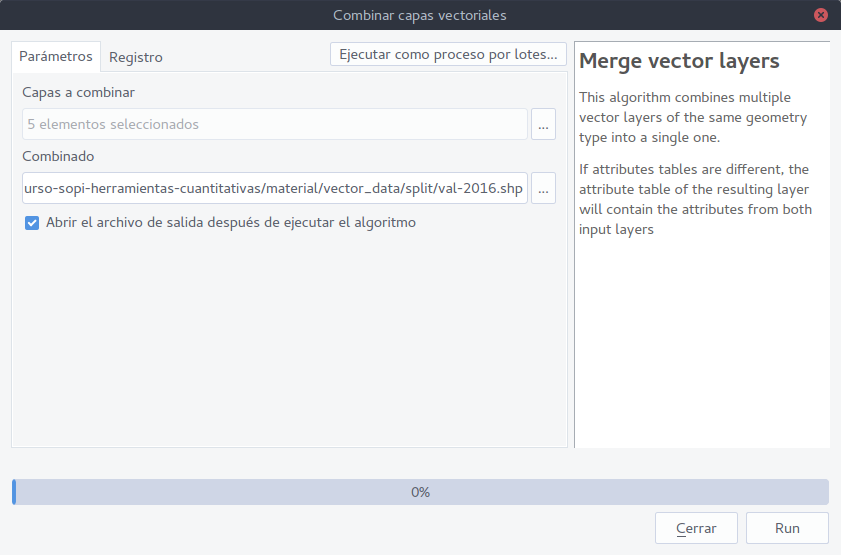
\includegraphics[scale=0.4]{combinar.png}
    \caption{Combinacion de poligonos en una capa vectorial.}
    \label{fig:combinar}
  \end{figure}

  Luego editamos su tabla de atributos para agregar el campo \verb|MC_ID| y, realizando un an\'alisis visual en distintas combinaciones de bandas, asignamos a cada punto el \verb|MC_ID| de la clase de informaci\'on a la que pertenece.

  Podemos utilizar la misma imagen que usamos para clasificar o una de mayor resoluci\'on espacial. Una vez terminada y guardada tendremos nuestra capa de validaci\'on.

\end{exa}

\begin{act}
  Construya de esta forma una serie de puntos de validaci\'on para la imagen Landsat 7 del a\~no 2000.
\end{act}

\begin{exa}

  Una vez obtenidos los puntos de validaci\'on podemos calcular la matriz de confusi\'on.  Para esto debemos cargar el pol\'igono de validaci\'on y la calculamos con la funci\'on \texttt{validateMap}.

  \begin{lstlisting}
      valid.2016 <- readOGR(dsn="vector_data", layer="validacion")
      val.2016 <- validateMap(mlc.3x3.2016,valData = valid.2016,
                                responseCol = "MC_ID")
  \end{lstlisting}

  Al inspeccionar el elemento \verb|val.2016$performance| obtenemos la matriz
  de confusi\'on, la presici\'on global como \emph{Acuracy}, la presici\'on del
  productor como \emph{Sensitivity} y la del usuario como \emph{Pos Pred Value}.

  \begin{Verbatim}[fontsize=\small]
    Confusion Matrix and Statistics

              Reference
    Prediction   1   2   5   7   8
             1 150  27  14   6   2
             2   5 164   0   0   0
             5   6   0  21   0   0
             7   1   0   0  35   5
             8   3   0   0   6  54

    Overall Statistics

                   Accuracy : 0.8497
                     95% CI : (0.8153, 0.8799)
        No Information Rate : 0.3828
        P-Value [Acc > NIR] : < 2.2e-16

                      Kappa : 0.7888
     Mcnemar's Test P-Value : NA

    Statistics by Class:

                         Class: 1 Class: 2 Class: 5 Class: 7 Class: 8
    Sensitivity            0.9091   0.8586  0.60000  0.74468   0.8852
    Specificity            0.8533   0.9838  0.98707  0.98673   0.9795
    Pos Pred Value         0.7538   0.9704  0.77778  0.85366   0.8571
    Neg Pred Value         0.9500   0.9182  0.97034  0.97380   0.9839
    Prevalence             0.3307   0.3828  0.07014  0.09419   0.1222
    Detection Rate         0.3006   0.3287  0.04208  0.07014   0.1082
    Detection Prevalence   0.3988   0.3387  0.05411  0.08216   0.1263
    Balanced Accuracy      0.8812   0.9212  0.79353  0.86570   0.9323
  \end{Verbatim}

  Una vez obtenida la matriz de confusi\'on y las superficies mediante el comando \texttt{freq()}, podemos usar el script de R \file{areas.R}. Nos devolver\'a un archivo csv con las superficies de cada categor\'ia de uso y cobertura, \emph{adj\_area}, y su error \emph{CI\_adj\_area} como se ve al ejecutar el comando \texttt{ov[c(1:5,11,12)]}.
  \begin{Verbatim}[fontsize=\small]
          1     2     5     7     8  adj_area CI_adj_area
    1 0.318 0.053 0.030 0.013 0.004 135500.03   11289.281
    2 0.015 0.488 0.000 0.000 0.000 215369.55    9285.073
    5 0.006 0.001 0.021 0.000 0.000  20265.40    6243.584
    7 0.000 0.000 0.000 0.016 0.003  12318.18    4174.173
    8 0.002 0.000 0.000 0.003 0.028  13907.63    2694.601
  \end{Verbatim}
\end{exa}


\begin{act}
    Construya la matriz de confusi\'on y obtenga la presici\'on global para todas las clasificaciones del a\~no 2000 y 2016. ¿Qu\'e algor\'itmo funciona mejor? Obtenga estimaciones de las superficies para los a\~nos 2000 y 2016 y util\'icela para estimar la perdida de selva paranaense durante este per\'iodo.
\end{act}
